\section{Problem}
\label{sec:problem}
We start by describing the problem addressed in this paper, including the problem definition and mathematical formulation. Then, we will give the proof that the problem is NP-hard.
\subsection{Problem Formulation}
In this paper, we consider the problem of designing the bin with least surface area that could pack all the items. %In a typical 3D-BPP, a set of items must be packed into fixed-sized bins in the way that minimizes the number of bins used. Unlike typical BPP with fixed-sized bins, we focus on the problem of designing the bin with least surface area that could pack all the items. 
\KZ{Did you mean cross-border e-commerce?}
In real business scenarios, such as cross-border e-commerce, packages should be packed with plastic wrapping as outer packaging before shipping. The goal of this scenario is to minimize the  packing materials per order by generating a better packing solution. 
After stacking all the items, the plastic wrapping can be formalized into a rectangular-shaped bin. As the result, the cost of this material is directly proportional to the surface area of the rectangular-shaped bin. In this case, minimizing the surface area for the bin would bring huge economic benefits.

The exact formulation of our 3D-FBPP is shown below. Given a set of cuboid-shaped items and each item $i$ is characterized by length ($l_i$), width ($w_i$) and height ($h_i$). Our target is to find the least-surface-area bin that can pack all items. 
Generally, we use $(x_i, y_i, z_i)$ to denote the front-left-bottom (FLB) coordinate of item $i$ and assume that FLB corner of the bin is $(0,0,0)$.  
%The details of decision variables are shown in Table \ref{variable table}. 
%\kz{It might be better to have a 3D illustration figure to help explain the constraints in the problem def.}
To ensure that there is no overlap, binary variables $s_{ij}$, $u_{ij}$, $b_{ij}$ are defined to indicate the placement of items $i$ to each item $j$. Variables will be 1 if items $i$  is in left of, under of, or on back of item $j$, respectively; otherwise, 0. The variable ${\delta}_{i1}$(resp. ${\delta}_{i2}$, ${\delta}_{i3}$, ${\delta}_{i4}$, ${\delta}_{i5}$, ${\delta}_{i6}$) is equal to 1 if the orientation of item $i$ is front-up (resp. front-down, side-up, side-down, bottom-up, bottom-down). Consequently, our aim is to find a least-surface-area bin of which the size is $(L,W,H)$, where $L$, $W$ and $H$ are the length, width and height of the bin, respectively. 

Based on the descriptions of problem and notations, the mathematical formulation for the 3D-FBPP follows that of \cite{hifi2010linear}:
\begin{eqnarray*}
	\begin{split}
		%\vspace{-100pt}
		%\begin{align*}
		&\min\,\,  L \cdot W + L \cdot H + W \cdot H\\ 
		&\texttt{s}.\texttt{t}.
		\begin{cases}
			s_{ij}+ u_{ij} + b_{ij}  =1          &(1)  \\ %&  i < j = 1,\dots,n    \\
			{\delta}_{i1} + {\delta}_{i2} + {\delta}_{i3} + {\delta}_{i4} + {\delta}_{i5} + {\delta}_{i6} =1  & (2)   \\ 
			x_i - x_j + L  \cdot  s_{ij}  \le  L - \hat{l_i}                           & (3)  \\ %&  i < j = 1,\dots,n \\
			y_i - y_j + W \cdot b_{ij} \le W - \hat{w_i}                        & (4)   \\ %&  i < j = 1,\dots,n \\
			z_i - z_j + H \cdot u_{ij} \le  H - \hat{h_i}                                                                                   & (5)    \\ %&  i < j = 1,\dots,n\\
			0 \le x_i \le L- \hat{l_i}                                     & (6)\\ %&    i = 1,\dots , n      \\
			0 \le y_i \le W - \hat{w_i}                                 & (7)\\ %&      i = 1,\dots , n \\
			0 \le z_i \le H - \hat{h_i}                                   & (8)\\ %&     i = 1,\dots , n  \\
			\hat{l_i} = {\delta}_{i1}   l_i + {\delta}_{i2}  l_i + {\delta}_{i3}  w_i + {\delta}_{i4}  w_i + {\delta}_{i5}  h_i + {\delta}_{i6}  h_i& (9)\\   %&     i = 1,\dots , n \\
			\hat{w_i} = {\delta}_{i1}  w_i +{\delta}_{i2}  h_i +{\delta}_{i3}  l_i +{\delta}_{i4}  h_i +{\delta}_{i5}  l_i +{\delta}_{i6}  w_i& (10)\\ %&     i = 1,\dots , n  \\
			\hat{h_i} =  {\delta}_{i1}  h_i +{\delta}_{i2}  w_i +{\delta}_{i3}  h_i +{\delta}_{i4}  l_i + {\delta}_{i5}  w_i +{\delta}_{i6}  l_i& (11)\\%&     i = 1,\dots , n\\
			s_{ij} , u_{ij},  b_{ij}  \in \{0,1\}                                                                                                                      & (12)\\%&  i < j = 1,\dots,n  \\
			{\delta}_{i1}, {\delta}_{i2}, {\delta}_{i3}, {\delta}_{i4}, {\delta}_{i5}, {\delta}_{i6} \in \{0,1\}                                                     &(13)\\
		\end{cases}
		%\vspace{-20pt}
	\end{split}
\end{eqnarray*}

Constraints $(9)-(11)$ denote the actual length, width, height of item $i$ after orientating it. Constraints $(1)-(5)$ are used to guarantee there is no overlap between two packed items while constraints $(6)-(8)$ are used to guarantee the item will not be put outside the bin. Figure \ref{fig:problem-illu} explains the non-overlapping constraints in the problem definition.

\begin{figure}[h]
	\centering
	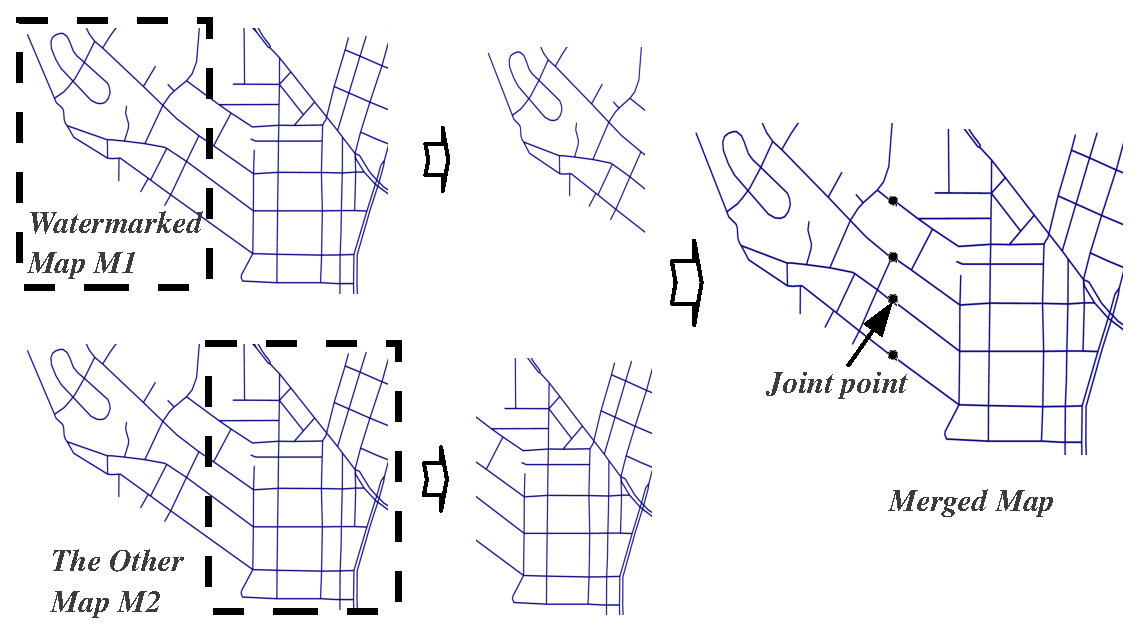
\epsfig{file=problem.png, width=0.65\columnwidth}
	\caption{Illustration of non overlapping constraint: item 1 is under item 2 and this means $u_{1,2}=1$ and $z_1 + h_1 <= z_2$, which is constraint (5); item 1 is in the left of item 3 and this means $s_{1,3}=1$ and $x_1 + l_1 <= x_3$, which is constraint (3). }
	\label{fig:problem-illu}
	\vspace{-15pt}
\end{figure}
\subsection{Proof of NP-hardness}

\textbf{Lemma 1.} \textit{Two-dimensional flexible bin packing problem (2D-FBPP) is NP-hard.}

\hspace{-1em}Proof. Given a one-dimensional bin packing problem (1D-BPP) that consists of $n$ items $I=\{(w_i)\}_{i=1}^{n}$ with integer size and bins with integer capacity $W$, we can reduce it to 2D-FBPP. The transformed 2D-FBPP involves $n$ items $I^{'}=\{(1/(n \cdot max({w_i})),w_i\}_{i=1}^{n}$ and a base item $B=(W \cdot n \cdot max(x_i),W)$. The 2D-FBPP is to find the bin with least surface area to pack all items, whereas 1D-BPP aims to minimize the number of bins used.  

Without loss of generality, we assume the base item $B$ is on the left-bottom of the bin. The remaining $n$ items could be put on the right side or on the upper side of $B$. The exactly increased area is $W\cdot K/(n\cdot max(w_i))$ when packing all items on the right, while the least increased area $A^{'}$ in other situations is as follows:
$$A^{'}=
\begin{cases}
W, \qquad\qquad\quad \text{pack one item on the upper side}\\
W \cdot min(w_i), \ \ \text{rotate and pack one item on the right} \\
%W/(max(w_i)),\quad \text{pack all items on the right}
\end{cases}
$$ 
where $K$ is an integer and $K<=n$. Thus, all the items must be put on the right side of $B$ and tightly packed without any rotation. In 1D-BPP, $K$ can be treated as the number of bin used. In that case, to find a bin with least surface area for this $n+1$ items is equal to find the least number of bins of capacity $W$ for items $I$. Therefore, if we can solve the 2D-FBPP in polynomial time, the 1D-BPP can be solved in polynomial time, which completes the proof that this 2D-FBPP is NP-hard unless $P = NP$.

%Moreover, to obtain less surface area, all items must be tightly packed like Figure \ref{fig:nphard}b. If rotating one item, the total increased area is at least $W \cdot min(w_i)$. Intuitively, all items must be tightly packed like Figure \ref{fig:nphard}b for the purpose of less surface area, and increased area is $[W*K/(n.max(w_i)),W/max(w_i)]$ where 


%\begin{figure}[h]
%	\centering
%	\epsfig{file=nphard1.png, width=0.80\columnwidth}
%	\caption{Illustration of the placement of the n-remaining items. (a) shows that items packed on the right is not appropriate, which increases the surface area $(W \cdot n \cdot max(x_i) )/( n \cdot max(w_i))=W$ at least and stacking all items vertically on the top increases the surface area less than $W$; (b) shows the most appropriate packing pattern for all $n$ items. }
%	\label{fig:nphard}
%	\vspace{-10pt}
%\end{fi gure}

%\begin{theorem}
%  3D-FBPP is NP-hard.	
%\end{theorem}
\hspace{-1em}\textbf{Theorem 1.} \textit{3D-FBPP is NP-hard.}
%\begin{proof}
%For 3D-FBPP, we will add height $1/(n \cdot max({w_i}))^2$ for each item in the 2D case, which will ensure no item will be placed on the height side. Proof is the same as the 2D case.
%\end{proof}

\hspace{-1em}Proof. For 3D-FBPP, we will add the third dimension $1/(n \cdot max({w_i}))^2$ for each item in the 2D case, which will ensure no item will be placed on the third dimension. Proof is the same as the 2D case.

%In addition to proving that this 3D-FBPP is NP-hard, we have tried to solve the problem by optimization solvers, such as Gurobi\footnote{\url{ http://www.gurobi.com}}, but since its Hessian matrix is not positive or semi-determined, it cannot be solved directly.
